\documentclass[12pt]{article}
\usepackage[margin=0.85in]{geometry}
\usepackage{booktabs,longtable,array}
\usepackage{xcolor}
\usepackage{hyperref}
\usepackage{pdfpages}
\hypersetup{colorlinks=true,linkcolor=blue,urlcolor=blue}
\emergencystretch=2em

% Suite report typography. Keep a local copy for standalone portability.
% Build with LuaLaTeX and an installed, genuine Times New Roman font family.
\usepackage{fontspec}
\setmainfont{Times New Roman}
\usepackage{ragged2e,titlesec,caption,etoolbox}
\titleformat{\section}{\normalfont\bfseries\fontsize{15}{17}\selectfont\raggedright}{\thesection}{0.6em}{}
\titleformat{\subsection}{\normalfont\bfseries\fontsize{15}{17}\selectfont\raggedright}{\thesubsection}{0.6em}{}
\titleformat{\subsubsection}{\normalfont\bfseries\fontsize{15}{17}\selectfont\raggedright}{\thesubsubsection}{0.6em}{}
\titleformat{\paragraph}[runin]{\normalfont\bfseries\fontsize{15}{17}\selectfont}{\theparagraph}{0.6em}{}
\DeclareCaptionFont{reporttext}{\normalfont\rmfamily\fontsize{12}{14}\selectfont}
\captionsetup{font=reporttext,labelfont=normalfont,textfont=normalfont,justification=justified,singlelinecheck=false}
\makeatletter
\renewcommand{\normalsize}{\@setfontsize\normalsize{12}{14}\abovedisplayskip=8pt plus 2pt minus 4pt\belowdisplayskip=8pt plus 2pt minus 4pt\abovedisplayshortskip=0pt plus 2pt\belowdisplayshortskip=5pt plus 2pt minus 2pt}
% Tables may be compact, but never below 10 pt or scaled down as graphics.
\renewcommand{\small}{\@setfontsize\small{10}{12}}
\renewcommand{\footnotesize}{\@setfontsize\footnotesize{10}{12}}
\renewcommand{\scriptsize}{\@setfontsize\scriptsize{10}{12}}
\renewcommand{\tiny}{\@setfontsize\tiny{10}{12}}
\renewcommand{\maketitle}{\par\begingroup\raggedright\normalfont\bfseries\fontsize{15}{17}\selectfont\@title\par\endgroup\vspace{12pt}}
\makeatother
\setlength{\emergencystretch}{3em}
% Consistent article paragraphs in every standalone case and guide narrative.
\setlength{\parindent}{15pt}
\setlength{\parskip}{0pt plus 1pt}
\linespread{1}
% Body prose in individual reports and aggregate summaries is always 12 pt.
\newcommand{\ReportBodyText}{\normalfont\normalsize\justifying}
\AtBeginDocument{\ReportBodyText}

\begin{document}
\newcommand{\GuideTitle}{ELMFIRE Validation Guide}
% Generated by tools/generate_summary_reports.py; do not edit by hand.
\newcommand{\AggregateELMFIREVersion}{not declared}

% Report cover: title only, with no subtitle, author block, or date.
\hypersetup{pageanchor=false}
\begin{titlepage}
  \thispagestyle{empty}
  \raggedleft

  \vspace*{0.09\textheight}
  {\color{blue!65!black}\rule{0.82\textwidth}{1.2pt}\par}
  \vspace{1.25cm}

  {\Huge\bfseries
    \GuideTitle\par}

  \vspace{1.1cm}
  {\large\bfseries Authors\par}
  \vspace{0.3cm}
  {\normalsize
    \renewcommand{\arraystretch}{1.12}
    \begin{tabular}{r}
      Yiren Qin \\
      Nikolaos Kalogeropoulos \\
      Daniel San Martin \\
      Adam Laird \\
      Dwi M. J. Purnomo \\
      Mateo Giorgi \\
      Maria Theodore \\
      Kasra Shamsaei \\
      Majid Bavandpour \\
      Arnaud Trouv\'e \\
      Michael J. Gollner \\
      Chris Lautenberger
    \end{tabular}\par
  }

  \vspace{0.75cm}
  {\large\bfseries Affiliations\par}
  \vspace{0.3cm}
  {\normalsize
    \renewcommand{\arraystretch}{1.18}
    \begin{tabular}{r}
      University of California, Berkeley \\
      Cloudfire Inc. \\
      University of Maryland, College Park \\
    \end{tabular}\par}

  \vfill
  {
    \renewcommand{\arraystretch}{1.35}
    \begin{tabular}{@{}r@{}}
      \textbf{ELMFIRE version:} \AggregateELMFIREVersion \\
      \textbf{Compiled:} \today \\
    \end{tabular}
    \par
  }

  \vspace{0.75cm}
  {\color{blue!65!black}\rule{0.82\textwidth}{1.2pt}\par}
  \vspace*{0.045\textheight}
\end{titlepage}
\hypersetup{pageanchor=true}
\pagenumbering{arabic}


\section*{About This Guide}
\phantomsection
\addcontentsline{toc}{section}{About This Guide}
This guide compares ELMFIRE predictions with observations for the active
validation cases. Each report describes the event, input data, modeling choices,
comparison methods, and uncertainties. The opening summary presents the
calculated decisions and the computational information available during report
preparation. A completed simulation does not by itself establish validation.

\clearpage
\tableofcontents
\clearpage

\section{How to Read This Guide}

Start with the validation summary for the recorded computational environment,
declared parallel allocation, and scientific decision table. The
case identifiers in the summary link to the corresponding case-report entries.
The common landscape-validation evidence then explains the metrics and
limitations shared by the current cases, followed by each complete standalone
case report with its event-specific provenance, configuration, figures,
results, and limitations.

Interpret PASS and FAIL only where a case defines a justified acceptance
decision.  CHARACTERIZED means that descriptive metrics exist without a
justified pass threshold.  Missing, unrun, incomplete, or otherwise
non-decisional evidence is shown as NOT EVALUABLE. A completed narrative alone
does not establish validation evidence. The environment recorded during report
preparation is not necessarily the
execution environment of every included case.

% Generated by tools/generate_summary_reports.py; do not edit by hand.
\clearpage
\section{Validation summary}
\label{sec:validation-summary}
\ReportBodyText
\subsection{Computational environment recorded during report preparation}
The following information describes the environment available during preparation of this guide. It does not establish the environment used for earlier simulations. An available compiler is not necessarily the compiler used to build the model. ELMFIRE was not executed to obtain these observations; an undeclared model release remains unknown.

\begingroup\small
\begin{longtable}{@{}>{\raggedright\arraybackslash}p{0.27\textwidth}>{\raggedright\arraybackslash}p{0.68\textwidth}@{}}
\toprule
Configuration & Recorded value \\
\midrule
\endfirsthead
\toprule
Configuration & Recorded value \\
\midrule
\endhead
\bottomrule
\endlastfoot
Recorded at (Coordinated Universal Time) & 2026-09-15T18:02:20+00:00 \\
Declared ELMFIRE release & not declared \\
Operating system & macOS-15.7.7-arm64-arm-64bit \\
Processor architecture & arm64 \\
Message Passing Interface (MPI) implementation & not available \\
Available Fortran compiler & GNU Fortran (Homebrew GCC 14.2.0\_1) 14.2.0 \\
Python version & CPython 3.12.9 \\
Scientific analysis libraries & NumPy 1.26.4; \allowbreak{}Matplotlib 3.9.2; \allowbreak{}PyYAML 6.0.1; \allowbreak{}Rasterio 1.5.0; \allowbreak{}GDAL not installed; \allowbreak{}Pandas 2.2.2; \allowbreak{}GeoPandas not installed; \allowbreak{}Shapely not installed \\
\end{longtable}
\endgroup\ReportBodyText

\subsection{Comparison type and declared parallel allocation}
The comparison type distinguishes isolated and coupled processes or the spatial scale of validation. The process count is the allocation declared for each case, not a measurement of resources used in an earlier simulation. Missing declarations are not inferred.

\begingroup\scriptsize
\begin{longtable}{@{}>{\raggedright\arraybackslash}p{0.22\textwidth}>{\raggedright\arraybackslash}p{0.48\textwidth}>{\raggedright\arraybackslash}p{0.20\textwidth}@{}}
\toprule
Case & Comparison type & MPI processes \\
\midrule
\endfirsthead
\toprule
Case & Comparison type & MPI processes \\
\midrule
\endhead
\midrule
\multicolumn{3}{r}{Continued on next page} \\
\endfoot
\bottomrule
\endlastfoot
\hyperref[case-detail:camp-fire]{camp\_fire} & Landscape-scale validation & 50 \\
\hyperref[case-detail:thomas-fire]{thomas\_fire} & Landscape-scale validation & 50 \\
\hyperref[case-detail:tubbs-fire]{tubbs\_fire} & Landscape-scale validation & 50 \\
\end{longtable}
\endgroup\ReportBodyText

\subsection{Scientific decision summary}
The decisions below follow the established calculated metrics and case-specific acceptance criteria. Completing a simulation or preparing a report does not establish PASS. Missing or insufficient scientific evidence is reported as NOT EVALUABLE.

\textbf{Total cases:} 3\quad
\textbf{PASS:} 0\quad
\textbf{FAIL:} 0\quad
\textbf{CHARACTERIZED:} 3\quad
\textbf{NOT EVALUABLE:} 0

\begingroup\small
\setlength{\LTpre}{0.8em}
\setlength{\LTpost}{0pt}
\begin{longtable}{@{}>{\raggedright\arraybackslash}p{0.15\textwidth}>{\raggedright\arraybackslash}p{0.16\textwidth}>{\raggedright\arraybackslash}p{0.38\textwidth}>{\raggedright\arraybackslash}p{0.22\textwidth}@{}}
\toprule
Case & Category & Title & Decision \\
\midrule
\endfirsthead
\toprule
Case & Category & Title & Decision \\
\midrule
\endhead
\midrule
\multicolumn{4}{r}{Continued on next page} \\
\endfoot
\bottomrule
\endlastfoot
\hyperref[case-detail:camp-fire]{camp\_fire} & Landscape-scale validation & \hyperref[case-detail:camp-fire]{2018 Camp Fire landscape reconstruction} & \mbox{\textcolor{blue!70!black}{\textbf{CHARACTERIZED}}} \\
\hyperref[case-detail:thomas-fire]{thomas\_fire} & Landscape-scale validation & \hyperref[case-detail:thomas-fire]{2017 Thomas Fire landscape reconstruction} & \mbox{\textcolor{blue!70!black}{\textbf{CHARACTERIZED}}} \\
\hyperref[case-detail:tubbs-fire]{tubbs\_fire} & Landscape-scale validation & \hyperref[case-detail:tubbs-fire]{2017 Tubbs Fire landscape reconstruction} & \mbox{\textcolor{blue!70!black}{\textbf{CHARACTERIZED}}} \\
\end{longtable}
\endgroup\ReportBodyText

\begin{samepage}
\paragraph{Decision vocabulary.}
PASS and FAIL are case-defined scientific decisions. CHARACTERIZED denotes descriptive validation metrics without a justified acceptance threshold. NOT EVALUABLE denotes missing, unrun, incomplete, unsupported, or otherwise non-decisional evidence.
\end{samepage}


\section{Common landscape-validation evidence}

The current Camp, Thomas, and Tubbs landscape cases were reconstructed from the
supplied historical-fire datasets. Each is designed to
compare a 50-member ELMFIRE ensemble with cumulative Visible Infrared Imaging
Radiometer Suite (VIIRS) active-fire
detections.  The case reports retain the event-specific input provenance,
namelist rationale, evidence status, and unresolved limitations.

Their common spatial metrics are Jaccard overlap, precision, recall,
$F_1$, predicted-to-observed area ratio, and Brier score.  Together these
distinguish spatial mismatch, overgrowth, undergrowth, scale bias, and
probabilistic error.  Because the recovered archives define no acceptance
thresholds and do not quantify VIIRS-hull uncertainty, completed runs are
reported as CHARACTERIZED rather than PASS or FAIL unless justified thresholds
are declared before inspecting results.  Unresolved model-input provenance,
VIIRS collection or granule provenance, and event-specific calibration history
are stated explicitly in the standalone reports.

% Generated by tools/generate_summary_reports.py; do not edit by hand.
\clearpage
\IfFileExists{../cases/Validation/landscape_scale/camp_fire/report/case_report.pdf}{%
  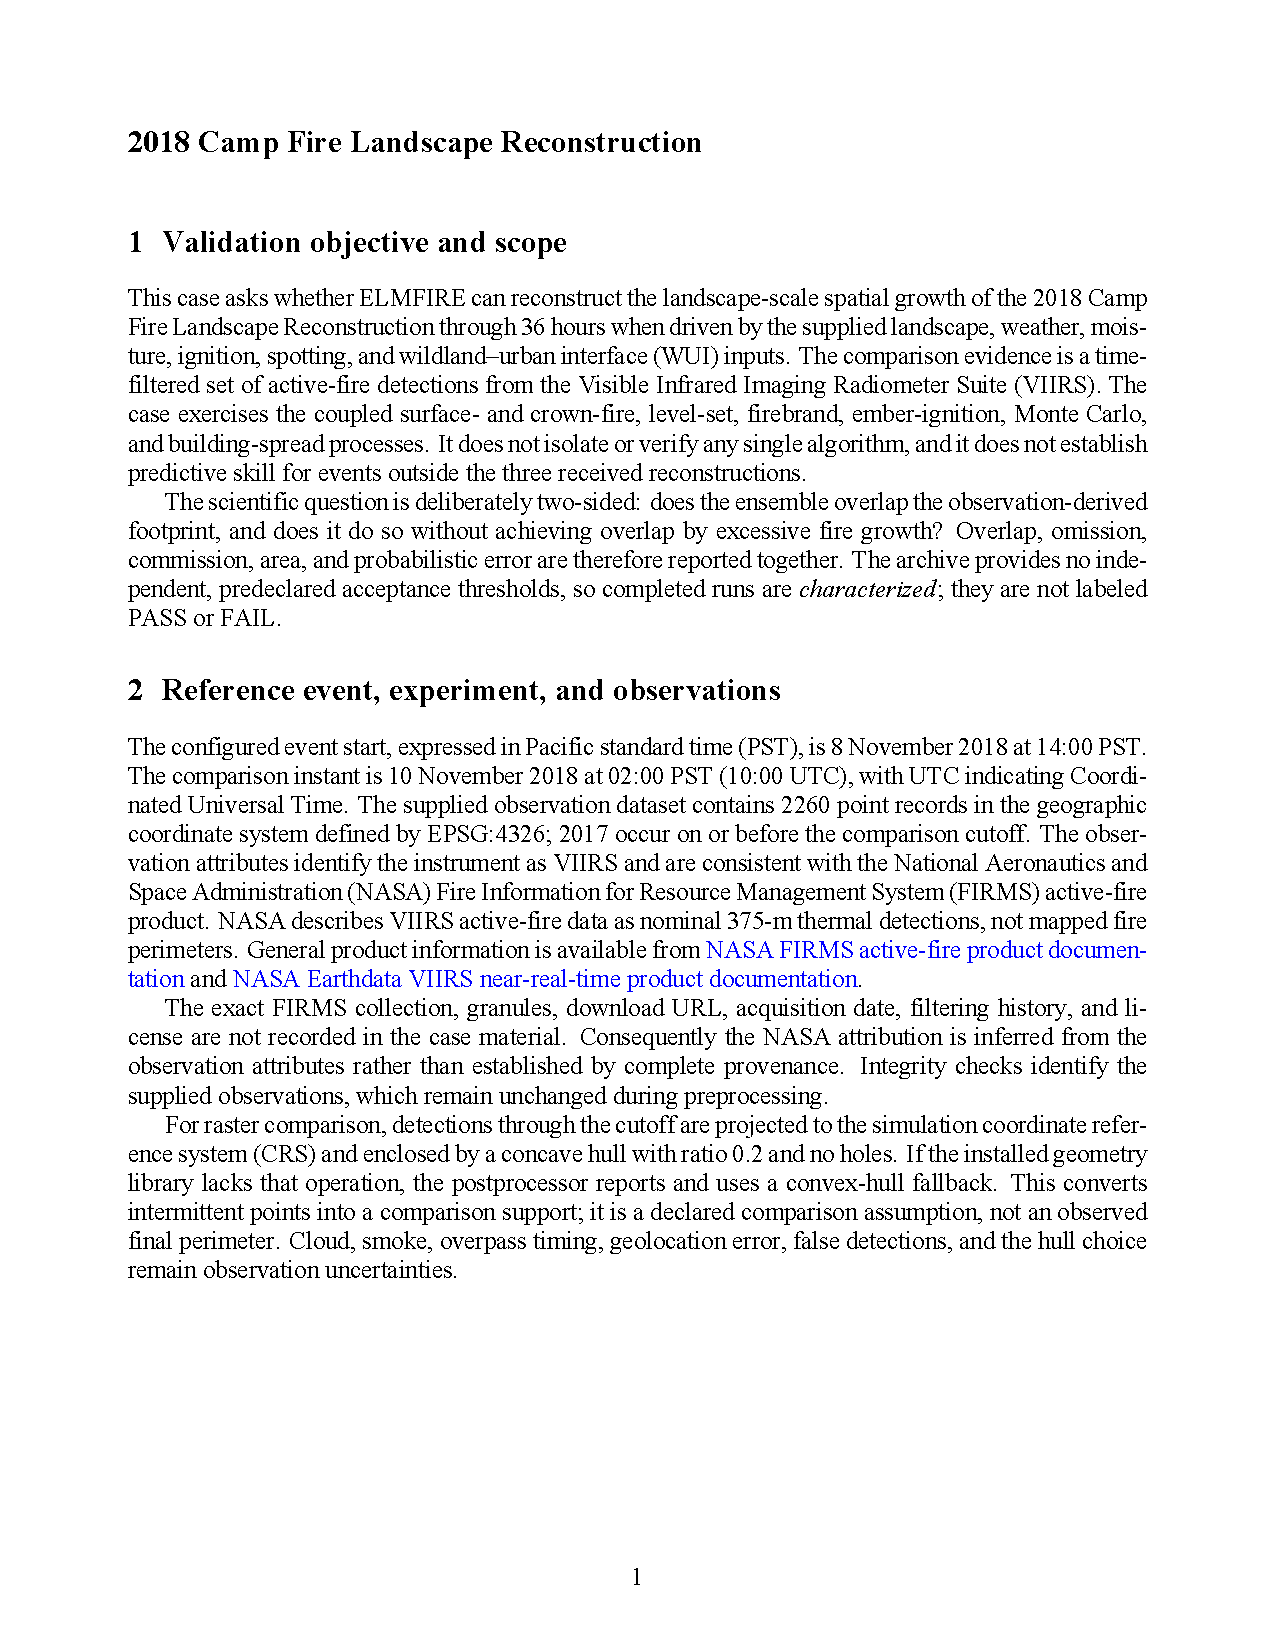
\includepdf[pages=-,pagecommand={\thispagestyle{empty}},addtotoc={1,section,1,{camp\_fire -- 2018 Camp Fire landscape reconstruction},case-detail:camp-fire}]{../cases/Validation/landscape_scale/camp_fire/report/case_report.pdf}%
}{%
  \phantomsection
  \label{case-detail:camp-fire}
  \addcontentsline{toc}{section}{camp\_fire -- 2018 Camp Fire landscape reconstruction}
  \section*{camp\_fire -- 2018 Camp Fire landscape reconstruction}
  \textbf{NOT EVALUABLE:} the detailed case description is unavailable.
}

\clearpage
\IfFileExists{../cases/Validation/landscape_scale/thomas_fire/report/case_report.pdf}{%
  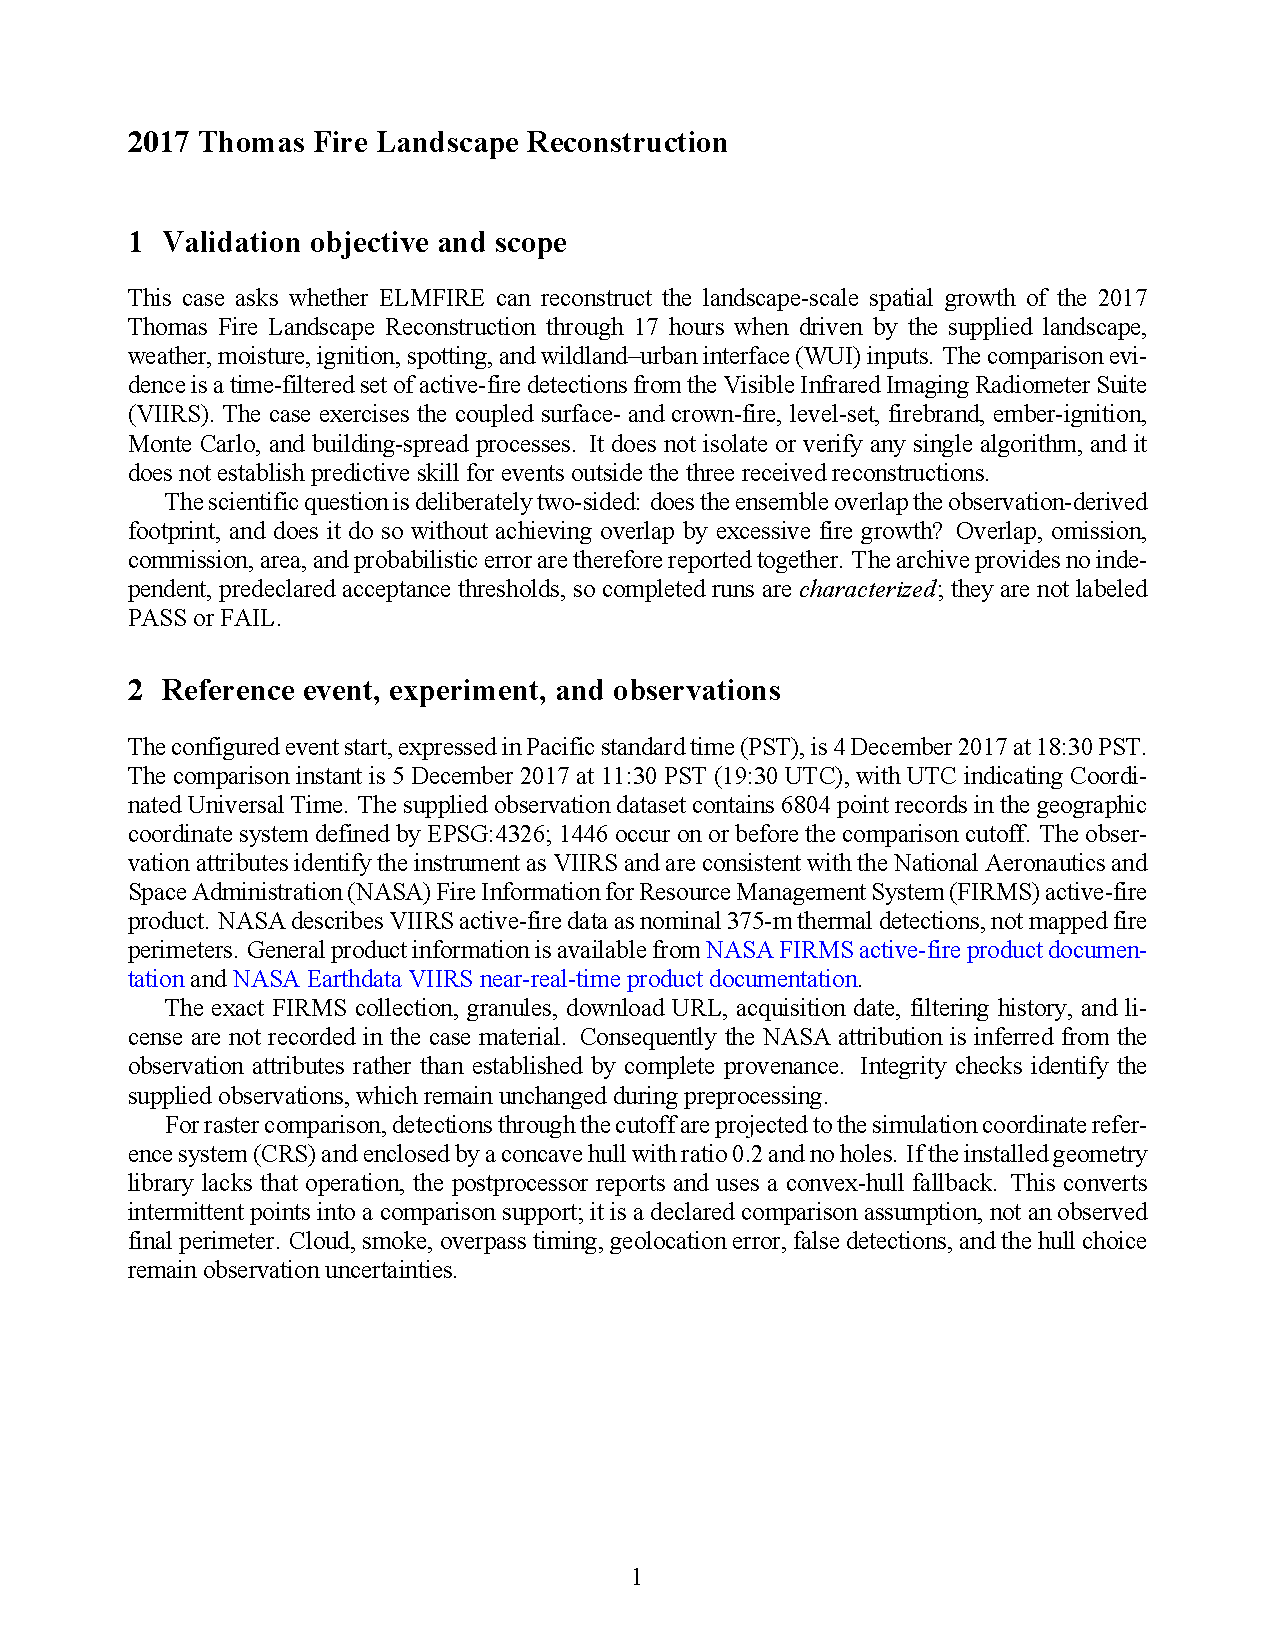
\includepdf[pages=-,pagecommand={\thispagestyle{empty}},addtotoc={1,section,1,{thomas\_fire -- 2017 Thomas Fire landscape reconstruction},case-detail:thomas-fire}]{../cases/Validation/landscape_scale/thomas_fire/report/case_report.pdf}%
}{%
  \phantomsection
  \label{case-detail:thomas-fire}
  \addcontentsline{toc}{section}{thomas\_fire -- 2017 Thomas Fire landscape reconstruction}
  \section*{thomas\_fire -- 2017 Thomas Fire landscape reconstruction}
  \textbf{NOT EVALUABLE:} the detailed case description is unavailable.
}

\clearpage
\IfFileExists{../cases/Validation/landscape_scale/tubbs_fire/report/case_report.pdf}{%
  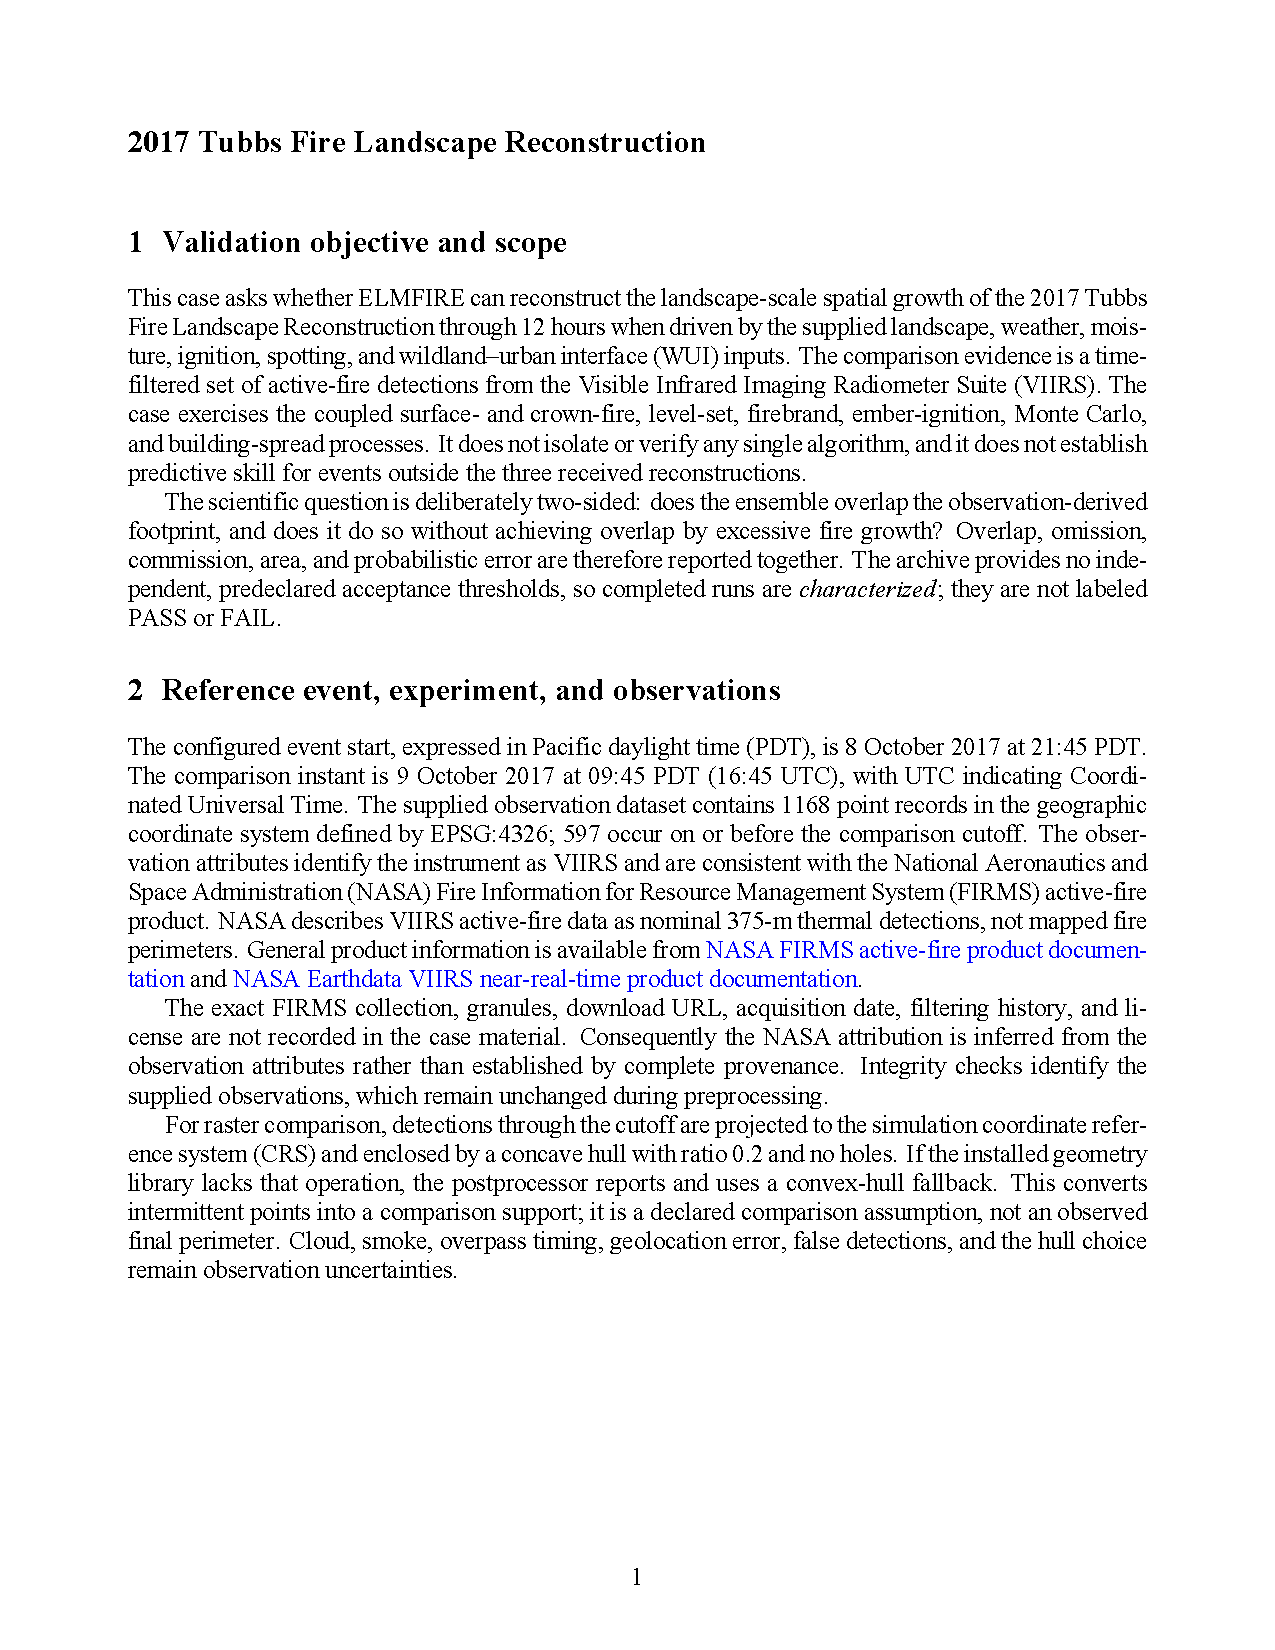
\includepdf[pages=-,pagecommand={\thispagestyle{empty}},addtotoc={1,section,1,{tubbs\_fire -- 2017 Tubbs Fire landscape reconstruction},case-detail:tubbs-fire}]{../cases/Validation/landscape_scale/tubbs_fire/report/case_report.pdf}%
}{%
  \phantomsection
  \label{case-detail:tubbs-fire}
  \addcontentsline{toc}{section}{tubbs\_fire -- 2017 Tubbs Fire landscape reconstruction}
  \section*{tubbs\_fire -- 2017 Tubbs Fire landscape reconstruction}
  \textbf{NOT EVALUABLE:} the detailed case description is unavailable.
}


\end{document}
